%% ----------------------------------------------------------------
\chapter{Specification}
%% ----------------------------------------------------------------
\label{chap:specification}
\section{Brief}
The original agreed project specification and plan, handed in on the first week of the project, was to design, build, and test an electronic module capable of capturing still images from an unmanned aerial vehicle (UAV) and transmitting the images to a ground station. The module must use the UAV autopilot’s low-bandwidth RS485 serial link (38.4 kBaud). A program must be written to interface with the base station software over a TCP/IP link, allowing image data to be received and then displayed to the user. The electronic module would be constructed using strip-boards and would later be implemented on PCB if time is available.


\section{Objectives} 
The aim of the project was to achieve the following criteria, which were also prioritized in order to ensure organized and efficient work: 

%|||||||||| maybe add some justification to the why things were certain priorities? ||||||||||||||


\begin{itemize}
	\item The image should be encoded in such a way that a low quality image will be available quickly, the quality of which would improve as more information is downloaded. [high priority]
	\item Minimise the time needed to download the images from the UAV to the base station. The time from the user’s prompt until the image has been fully downloaded will be measured against the theoretical 3 minutes necessary to transmit a full image without using any compression. The goal will be to obtain a full image in \textbf{less than 3 minutes.} [high priority]
	\item The module weight will be \textbf{less than 250g}. [medium priority]
	\item Image resolution of \textbf{$640\times480$}. [medium priority]
	\item Allow the user to perform the following actions on the UAV’s camera from the base station:
	\begin{itemize}
		\item Prompt the UAV to \textbf{capture and download an image}. [high priority]
		\item \textbf{Cancel} the downloading of any image while the image is being downloaded. [medium priority]
		\item \textbf{Resend} an image in case the current preview is corrupted. [low priority]
		\item \textbf{Interrupt} the download of an incomplete image and allow the user to save the incomplete image. [low priority]
		\item Select the \textbf{resolution settings} of the image. [low priority]
		\item Display a progress indicator which will show the percentage of the image datareceived, as well as a time estimate for the rest of the image to be downloaded. [low priority]
		\item The image capture will be triggered automatically by the UAV using triggers built into the autopilot. [low priority]
		\item Allow the user to command the image capture to \textbf{trigger periodically} over a \textbf{userspecified time interval} will be added if time permits. [low priority]
	\end{itemize}
	\item Images will be transmitted in \textbf{colour} as opposed to black and white. [low priority]
	\item The user should be able to select between a colour image and a black and white image. [low priority]
\end{itemize}


\section{Deliverables}
The deliverables which were planned to be produced by the end of the project to the customer include:
\begin{itemize}
	\item \underline{Hardware}: Camera module, constructed on PCB (if time permits, otherwise on strip-board),including layout designs.
	\item \underline{Software}: All firmware for the electronic module, and software on the base station for viewing images. The full source code and all executable files will be included.
	\item \underline{Documentation}: Technical and User Documentation. This includes all schematics related to hardware as well as all other documents concerning both the software and hardware delivered.
	\item \underline{Public repository}: The full source code, all schematics, and all documents concerning both the software and hardware will be included on a public repository so that the client may share this information with his clients.
\end{itemize}

\section{Block Diagram}

\begin{figure}[H]
        \centering
        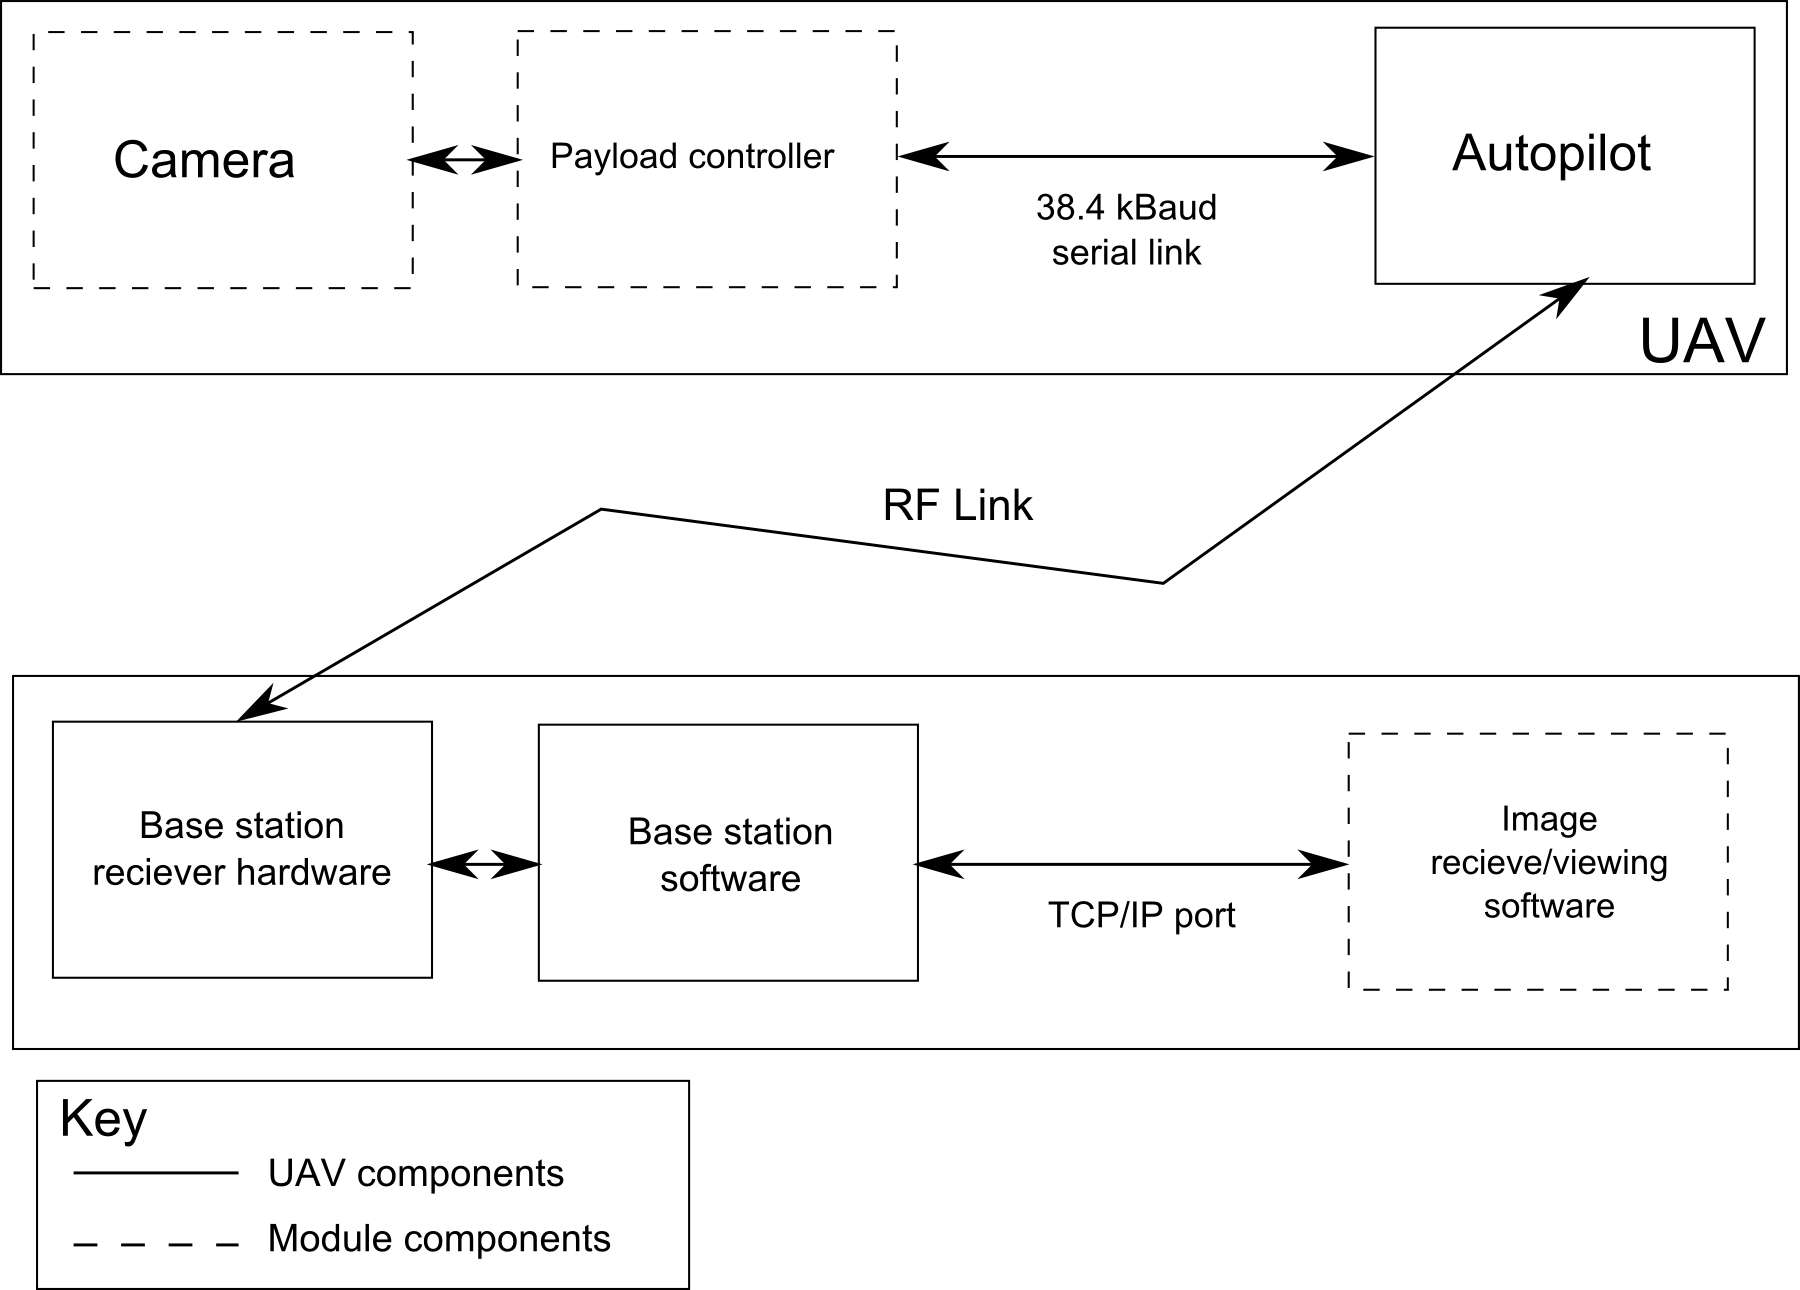
\includegraphics[width=1.00\textwidth]{figures/spec_block_diagram_2.png}
        \captionof{figure}{Block diagram of the specified system}
        \label{fig:block1}
\end{figure}

The above diagram (figure \ref{fig:block1}) gives an overview of how the system described in the specification all comes together. The parts with a solid outline are parts that we were given by our customer to fit our system around. The parts with the dashed outline are the elements of the design that we need to implement ourselves.

Inside the UAV itself will go the camera, the payload controller and the autopilot. The autopilot is provided by our customer and also provides our wireless link to the ground. The camera is simply a camera so that photographs can be taken. The payload controller is the part that needs the most work, it needs to be able to control the camera; take and get images as well as being able to communicate with the autopilot and interpret any commands sent up from the base station (also referred to as the ground station).

On the ground station side of things there is a radio frequency (rf) link to the autopilot (simulated by a USB cable for development purposes) which attaches to a computer running the ground station software provided by our customer. The ground station software provides two TCP/IP ports as interfaces, one for sending commands to the ground station software and to the autopilot and one for streaming data from the autopilot. It is these TCP/IP ports that our software on the ground has to interface with so that it can send commands up to the payload controller and then receive and display an image.
